% Options for packages loaded elsewhere
\PassOptionsToPackage{unicode}{hyperref}
\PassOptionsToPackage{hyphens}{url}
\PassOptionsToPackage{dvipsnames,svgnames,x11names}{xcolor}
%
\documentclass[
  authoryear,
  preprint,
  3p]{elsarticle}

\usepackage{amsmath,amssymb}
\usepackage{lmodern}
\usepackage{iftex}
\ifPDFTeX
  \usepackage[T1]{fontenc}
  \usepackage[utf8]{inputenc}
  \usepackage{textcomp} % provide euro and other symbols
\else % if luatex or xetex
  \usepackage{unicode-math}
  \defaultfontfeatures{Scale=MatchLowercase}
  \defaultfontfeatures[\rmfamily]{Ligatures=TeX,Scale=1}
\fi
% Use upquote if available, for straight quotes in verbatim environments
\IfFileExists{upquote.sty}{\usepackage{upquote}}{}
\IfFileExists{microtype.sty}{% use microtype if available
  \usepackage[]{microtype}
  \UseMicrotypeSet[protrusion]{basicmath} % disable protrusion for tt fonts
}{}
\makeatletter
\@ifundefined{KOMAClassName}{% if non-KOMA class
  \IfFileExists{parskip.sty}{%
    \usepackage{parskip}
  }{% else
    \setlength{\parindent}{0pt}
    \setlength{\parskip}{6pt plus 2pt minus 1pt}}
}{% if KOMA class
  \KOMAoptions{parskip=half}}
\makeatother
\usepackage{xcolor}
\setlength{\emergencystretch}{3em} % prevent overfull lines
\setcounter{secnumdepth}{5}
% Make \paragraph and \subparagraph free-standing
\ifx\paragraph\undefined\else
  \let\oldparagraph\paragraph
  \renewcommand{\paragraph}[1]{\oldparagraph{#1}\mbox{}}
\fi
\ifx\subparagraph\undefined\else
  \let\oldsubparagraph\subparagraph
  \renewcommand{\subparagraph}[1]{\oldsubparagraph{#1}\mbox{}}
\fi


\providecommand{\tightlist}{%
  \setlength{\itemsep}{0pt}\setlength{\parskip}{0pt}}\usepackage{longtable,booktabs,array}
\usepackage{calc} % for calculating minipage widths
% Correct order of tables after \paragraph or \subparagraph
\usepackage{etoolbox}
\makeatletter
\patchcmd\longtable{\par}{\if@noskipsec\mbox{}\fi\par}{}{}
\makeatother
% Allow footnotes in longtable head/foot
\IfFileExists{footnotehyper.sty}{\usepackage{footnotehyper}}{\usepackage{footnote}}
\makesavenoteenv{longtable}
\usepackage{graphicx}
\makeatletter
\def\maxwidth{\ifdim\Gin@nat@width>\linewidth\linewidth\else\Gin@nat@width\fi}
\def\maxheight{\ifdim\Gin@nat@height>\textheight\textheight\else\Gin@nat@height\fi}
\makeatother
% Scale images if necessary, so that they will not overflow the page
% margins by default, and it is still possible to overwrite the defaults
% using explicit options in \includegraphics[width, height, ...]{}
\setkeys{Gin}{width=\maxwidth,height=\maxheight,keepaspectratio}
% Set default figure placement to htbp
\makeatletter
\def\fps@figure{htbp}
\makeatother

\usepackage{amsmath}
\usepackage{booktabs}
\usepackage{caption}
\usepackage{longtable}
\usepackage{setspace}
\doublespacing
\makeatletter
\makeatother
\makeatletter
\makeatother
\makeatletter
\@ifpackageloaded{caption}{}{\usepackage{caption}}
\AtBeginDocument{%
\ifdefined\contentsname
  \renewcommand*\contentsname{Table of contents}
\else
  \newcommand\contentsname{Table of contents}
\fi
\ifdefined\listfigurename
  \renewcommand*\listfigurename{List of Figures}
\else
  \newcommand\listfigurename{List of Figures}
\fi
\ifdefined\listtablename
  \renewcommand*\listtablename{List of Tables}
\else
  \newcommand\listtablename{List of Tables}
\fi
\ifdefined\figurename
  \renewcommand*\figurename{Figure}
\else
  \newcommand\figurename{Figure}
\fi
\ifdefined\tablename
  \renewcommand*\tablename{Table}
\else
  \newcommand\tablename{Table}
\fi
}
\@ifpackageloaded{float}{}{\usepackage{float}}
\floatstyle{ruled}
\@ifundefined{c@chapter}{\newfloat{codelisting}{h}{lop}}{\newfloat{codelisting}{h}{lop}[chapter]}
\floatname{codelisting}{Listing}
\newcommand*\listoflistings{\listof{codelisting}{List of Listings}}
\makeatother
\makeatletter
\@ifpackageloaded{caption}{}{\usepackage{caption}}
\@ifpackageloaded{subcaption}{}{\usepackage{subcaption}}
\makeatother
\makeatletter
\@ifpackageloaded{tcolorbox}{}{\usepackage[many]{tcolorbox}}
\makeatother
\makeatletter
\@ifundefined{shadecolor}{\definecolor{shadecolor}{rgb}{.97, .97, .97}}
\makeatother
\makeatletter
\makeatother
\journal{Quaternary Science Reviews}
\ifLuaTeX
  \usepackage{selnolig}  % disable illegal ligatures
\fi
\usepackage[]{natbib}
\bibliographystyle{elsarticle-harv}
\IfFileExists{bookmark.sty}{\usepackage{bookmark}}{\usepackage{hyperref}}
\IfFileExists{xurl.sty}{\usepackage{xurl}}{} % add URL line breaks if available
\urlstyle{same} % disable monospaced font for URLs
\hypersetup{
  pdftitle={Supplement of Hydroclimate variations over the last 17,000 years as estimated by leaf waxes in rodent middens from the south-central Atacama Desert, Chile},
  pdfauthor={Matías Frugone-Álvarez; Sergio Contreras; Oliver Meseguer-Ruiz; Eduardo Tejos; Antonio Delgado-Huertas; Blas Valero-Garcés; Francisca P. Díaz; Matías Briseño; Manuel Bustos-Morales; Claudio Latorre,},
  pdfkeywords={Leaf cuticular waxes, Rodent Middens, Atacama
Desert, Hydroclimate, Quaternary},
  colorlinks=true,
  linkcolor={blue},
  filecolor={Maroon},
  citecolor={Blue},
  urlcolor={Blue},
  pdfcreator={LaTeX via pandoc}}

\setlength{\parindent}{6pt}
\begin{document}

\begin{frontmatter}
\title{Supplement of \emph{Hydroclimate variations over the last 17,000
years as estimated by leaf waxes in rodent middens from the
south-central Atacama Desert, Chile}}
\author[1,2,3]{Matías Frugone-Álvarez%
\corref{cor1}%
}
 \ead{matutefrugone@gmail.com} 
\author[1,5]{Sergio Contreras%
\corref{cor1}%
}
 \ead{scontreras@ucsc.cl} 
\author[6]{Oliver Meseguer-Ruiz%
%
}

\author[1]{Eduardo Tejos%
%
}

\author[7]{Antonio Delgado-Huertas%
%
}

\author[8]{Blas Valero-Garcés%
%
}

\author[9,2,10]{Francisca P. Díaz%
%
}

\author[11]{Matías Briseño%
%
}

\author[11]{Manuel Bustos-Morales%
%
}

\author[11,9,3]{Claudio Latorre,%
\corref{cor1}%
}
 \ead{clatorre@bio.puc.cl} 

\affiliation[1]{organization={Universidad Católica de la Santísima
Concepción, Departamento de Química Ambiental},addressline={Alonso de
Ribera 2850},city={Concepción, Chile},postcode={4090541},postcodesep={}}
\affiliation[2]{organization={ANID-Millennium Science Initiative Nucleus
(AFOREST)},addressline={Vicuña Mackenna 4860, Macul},city={Santiago,
Chile},postcode={7820436},postcodesep={}}
\affiliation[3]{organization={ANID-Millennium Science Initiative Nucleus
(UPWELL)},addressline={Raúl Bitrán 1305},city={La Serena,
Chile},postcodesep={}}
\affiliation[4]{organization={Universidad Católica de la Santísima
Concepción, Departamento de Química Ambiental, Facultad de
Ciencias},addressline={Alonso de Ribera 2850},city={Concepción,
Chile},postcode={4090541},postcodesep={}}
\affiliation[5]{organization={Centro de Investigación en Biodiversidad y
Ambientes Sustentables (CIBAS)},addressline={Alonso de Ribera
2850},city={Concepción, Chile},postcodesep={}}
\affiliation[6]{organization={Universidad de Tarapacá, Departamento de
Ciencias Históricas y Geográficas},addressline={Luis Emilio Recabarren
2477},city={Iquique, Chile},postcode={1101783},postcodesep={}}
\affiliation[7]{organization={Instituto Andaluz de Ciencias de la Tierra
(CSIC-UGR)},addressline={Av. de las Palmeras, 4, 18100
Armilla},city={Granada, Spain},postcodesep={}}
\affiliation[8]{organization={Instituto Pirenaico de
Ecología-CSIC, Quaternary Paleoenvironments and Global
Change},addressline={Avda. Montañana, 1005},city={Zaragoza,
Spain},postcodesep={}}
\affiliation[9]{organization={Instituto de Ecología y Biodiversidad,
Chile},addressline={Las Palmeras 3425, Ñuñoa},city={Santiago,
Chile},postcode={7800024},postcodesep={}}
\affiliation[10]{organization={Pontificia Universidad Católica de
Valparaíso. Instituto de Geografía},addressline={Avenida Brasil
2241},city={Valparaíso, Chile},postcode={2362807},postcodesep={}}
\affiliation[11]{organization={Pontificia Universidad Católica de
Chile, Departamento de Ecología},addressline={Av. Libertador Bernardo
O'Higgins 340.},city={Santiago, Chile},postcodesep={}}
\affiliation[12]{organization={Pontificia Universidad Católica de
Chile, Departamento de Ecología-Centro UC Desierto de
Atacama},addressline={Av. Libertador Bernardo O'Higgins
340.},city={Santiago, Chile},postcodesep={}}

\cortext[cor1]{Corresponding author}










        
\begin{abstract}
Leaf cuticular waxes are one of the most important environment-plant
interaction structural systems that enable desert plants to withstand
extreme climatic conditions. We present a long chain \emph{n}-alkyl
lipids study in fresh plant leaves and rodent paleomiddens collected
along an elevational gradient in the south-central Atacama Desert of
Chile, covering six different vegetation physiognomies: Steppe
(4,500-4,000 m asl), Puna (4,000-3,300 m asl), Prepuna (3,300-2,400 m
asl), Absolute Desert (2,400-2,000 m asl), Desert (1,000-2,000 m asl),
and Coastal Desert (1,000-0 m asl). The 28 rodent paleoenvironments
analysed from Quebrada Incahuasi (25.6 \(^\circ\)S, 3,600 m asl) span
the last 17,000 years. The distribution of long-chain \emph{n}-alkanes
and \emph{n}-alkanoic acids varies among the dominant plant associations
of the Atacama Desert. These plants show a species-specific
chemotaxonomy linked to the climatic conditions. Furthermore,
differences in average chain length (ACL) and carbon preference index
(CPI) suggest that these plant communities have adapted to these extreme
environmental conditions. The sum of leaf wax \emph{n}-alkanes was
highest under wet conditions, while \emph{n}-alkanoic acids (between
\emph{n}-\(C_{24}\) and \emph{n}-\(C_{28}\)) increased with
hyperaridity. Similarly, analysis of \emph{n}-alkane time series from
paleomiddens showed that the greatest changes in leaf wax
\emph{n}-alkane distributions (ACL and CPI) corresponded to the greatest
increases in moisture during the Central Andean Pluvial Event (CAPE;
between 18 and 9 ka cal BP) and the Late Holocene. The shift in the
paleomidden \emph{n}-alkane distributions is corroborated by the
relative abundance of rainfall-dependent extra-local taxa. This is the
first study to report leaf wax content obtained from ancient rodent
middens, and shows promising results as a robust hydroclimate proxy for
the Atacama Desert region.
\end{abstract}





\begin{keyword}
    Leaf cuticular waxes \sep Rodent Middens \sep Atacama
Desert \sep Hydroclimate \sep 
    Quaternary
\end{keyword}
\end{frontmatter}
    \ifdefined\Shaded\renewenvironment{Shaded}{\begin{tcolorbox}[enhanced, interior hidden, borderline west={3pt}{0pt}{shadecolor}, boxrule=0pt, breakable, sharp corners, frame hidden]}{\end{tcolorbox}}\fi

\hypertarget{supplementary-result}{%
\section{Supplementary Result}\label{supplementary-result}}

\hypertarget{abundance-and-distribution-of-long-chain-n-alkane-and-n-alkanoic-acids-in-leaf-cuticular-waxes-in-plants-along-an-environmental-gradient-in-the-atacama-desert.}{%
\subsection{\texorpdfstring{Abundance and distribution of long-chain
\emph{n}-alkane and \emph{n}-alkanoic acids in leaf cuticular waxes in
plants along an environmental gradient in the Atacama
Desert.}{Abundance and distribution of long-chain n-alkane and n-alkanoic acids in leaf cuticular waxes in plants along an environmental gradient in the Atacama Desert.}}\label{abundance-and-distribution-of-long-chain-n-alkane-and-n-alkanoic-acids-in-leaf-cuticular-waxes-in-plants-along-an-environmental-gradient-in-the-atacama-desert.}}

Several studies have characterized the relationship between leaf wax
concentrations and environmental variables along elevational gradients
as an approach to understanding past climatic changes
\citep{cerda-penaMolecularNalkylLeaf2020, feakinsProductionLeafWax2016, jansenStraightchainLipidBiomarker2006, nieto-morenoElevationdependentChangesNalkane2016, shepherdEffectsStressPlant2006}.
We observe a high variability in the total abundance of wax chain
lengths within and between the vegetation belts. (Figure 1S and
Table~\ref{tbl-1} example). For leaf wax \emph{n}-alkanoic acids, the
species with higher total abundance were Ephedra sp, Junellia
seriphioides and Haplopappus rigidus, with intraspecific differences
ranging from 211 to 1615 ug/gdw for Ephedra sp (see Table~\ref{tbl-1}
example). Total \emph{n}-alkanoic acids abundances range from 375.88
ug/gdw in \emph{Junellia seriploide} (\(CPI_{median}\) = 8.29 \(\pm\)
1.6; \(ACL_{median}\) = 24.91 \(\pm\) 0.13) to 91.16 ug/gdw in Cristaria
integerrima (\(CPI_{median}\) = 5.8; \(ACL_{median}\) = 25.69). Total
\emph{n}-alkanes abundances range between 70 \(\pm\) 61 ug/gdw in
\emph{Ephedra} sp. (\(CPI_{median}\) = 8 \(\pm\) 4 ; \(ACL_{median}\) =
28.16 \(\pm\) 1.57) to 789.95 ug/gdw in \emph{Perityle emoryi}
(\(CPI_{median}\) = 14 ; \(ACL_{median}\) = 28). The distribution of the
chain lengths in Pappostipa frigida (Steppa, Puna and Prepuna) was
characterized by a higher abundance between
\emph{n}-\(C_{26}\)/\emph{n}-\(C_{27}\) and
\emph{n}-\(C_{30}\)/\emph{n}-\(C_{31}\) where the dominant carbon was
\emph{n}-\(C_{28}\)/\emph{n}-\(C_{29}\). \emph{Junellia seriphioides}
(Puna) has a higher abundance of chai\emph{n}-length between
\emph{n}-\(C_{20}\) to \emph{n}-\(C_{28}\) and \emph{n}-\(C_{21}\) to
\emph{n}-\(C_{33}\) carbon atoms in \emph{n}-alkanoic acids and
\emph{n}-alkanes, respectively. The dominant carbon length chain is
\emph{n}-\(C_{21}\) alkane, while in \emph{n}-alkanoic acids are
\emph{n}-\(C_{22}\), \emph{n}-\(C_{24}\) and \emph{n}-\(C_{28}\).
\emph{Haplopappus rigidus} (Puna and Prepuna) has a higher abundance of
chain-lengths between \emph{n}-\(C_{22}\)/\emph{n}-\(C_{23}\) to
\emph{n}-\(C_{30}\)/ \emph{n}-\(C_{31}\), \emph{n}-\(C_{23}\)
\emph{n}-alkane dominated the apolar lipid fractions while the polar
fractions were dominated by \emph{n}-\(C_{28}\) and \emph{n}-\(C_{30}\).
\emph{Aloysia deserticola} (Puna and Prepuna) produced relatively less
total long-chain \emph{n}-alkane than other species and has wider
distribution. The apolar lipid fractions were dominated by
\emph{n}-\(C_{27}\), \emph{n}-\(C_{29}\), \emph{n}-\(C_{31}\) and
\emph{n}-\(C_{33}\). In contrast, the polar fractions were less abundant
and well distributed along all carbon atom chain-lengths distributions
of fatty acid. \emph{Atriplex imbricata} (Prepuna and Hyperarid Desert),
has a higher abundance of chain-lengths between \emph{n}-\(C_{20}\) to
\emph{n}-\(C_{30}\) and \emph{n}-\(C_{25}\) to \emph{n}-\(C_{31}\)
carbon atoms, where \emph{n}-\(C_{27}\) alkane and \emph{n}-\(C_{28}\)
\emph{n}-alkanoic acid are the dominant carbon lengths chain.
\emph{Tiquilia atacamensis} (hyperarid zone) has wider and asymmetric
waxes distributions than other species ---from
\emph{n}-\(C_{18}\)/\emph{n}-\(C_{19}\) to
\emph{n}-\(C_{33}\)/\emph{n}-C34, respectively--- where the
\emph{n}-\(C_{27}\), \emph{n}-\(C_{29}\) and \emph{n}-\(C_{31}\) alkanes
and \emph{n}-\(C_{18}\), \emph{n}-\(C_{20}\), \emph{n}-\(C_{22}\) and
\emph{n}-\(C_{24}\) alkanoics acid were the waxes predominated with
\emph{n}-\(C_{29}\) and \emph{n}-\(C_{22}\) as the dominant carbon
length chains, respectively. \emph{Ephedra americana} has a higher
abundance of \emph{n}-alkanes and \emph{n}-alkanoic acid with
chain-lengths between \emph{n}-\(C_{21}\) to \emph{n}-\(C_{31}\) and
\emph{n}-\(C_{22}\) to \emph{n}-C32 carbon atoms, respectively. In
\emph{Ephedra americana}, the chain-lengths of \emph{n}-alkanes and
\emph{n}-alkanoic acid more abundant are the \emph{n}-\(C_{31}\) and
\emph{n}-\(C_{28}\) carbon atoms, respectively. In \emph{Nolana
aplocaryoides}, the \emph{n}-alkanes and \emph{n}-alkanoic acids of
higher abundances were the chain lengths \emph{n}-\(C_{25}\) to
\emph{n}-\(C_{31}\) and \emph{n}-\(C_{18}\) to \emph{n}-\(C_{28}\),
respectively, with \emph{n}-\(C_{29}\) and \emph{n}-\(C_{18}\) carbon
atoms the dominants. We only extracted the \emph{n}-alkanes in
\emph{Perityle emoryi}, the chain length distribution of this species
was between \emph{n}-\(C_{27}\) to \emph{n}-\(C_{31}\) where the
\emph{n}-\(C_{29}\) carbon atom is most abundant. In \emph{Cristaria
integerrima}, we only extracted the fatty acid where the chain length
distribution has between \emph{n}-\(C_{28}\) to \emph{n}-\(C_{20}\)
(Figure 1S).

\begin{figure}

{\centering 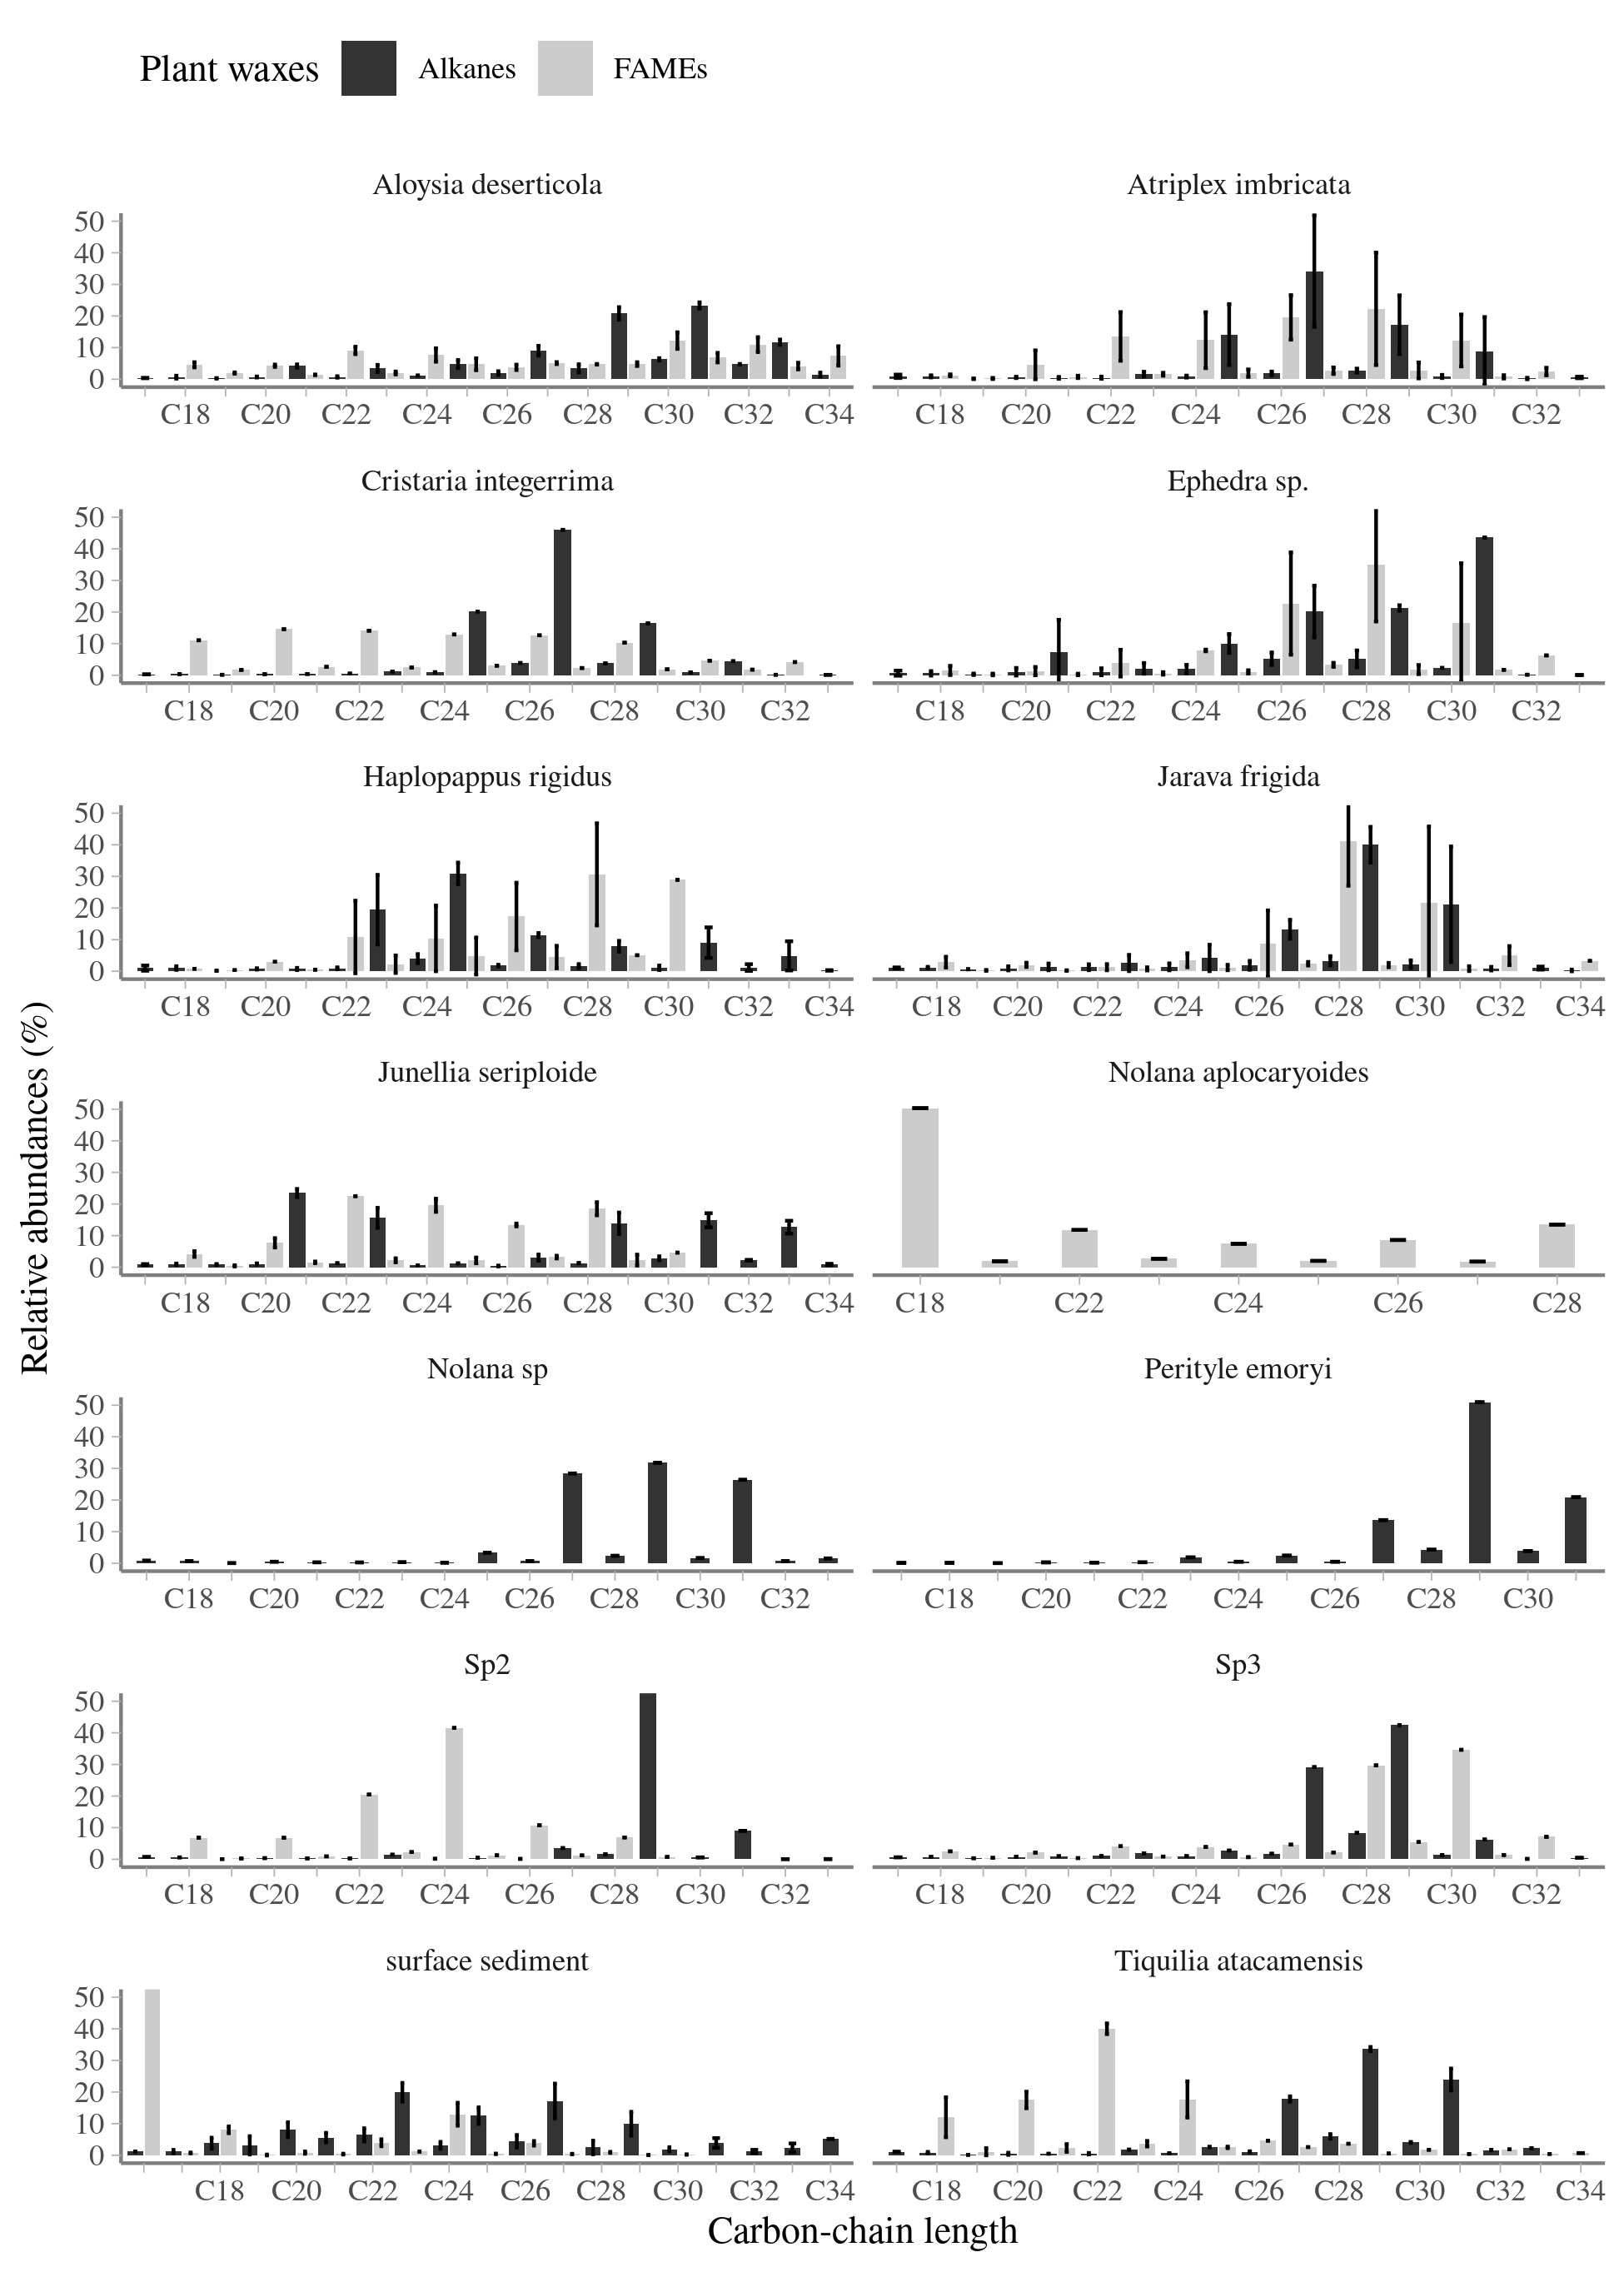
\includegraphics{images/Fig_1S.png}

}

\caption{Abundance of long-chain \emph{n}-alkane and \emph{n}-alkanoic
acids in leaf cuticular waxes by specie}

\end{figure}

\begin{figure}

{\centering 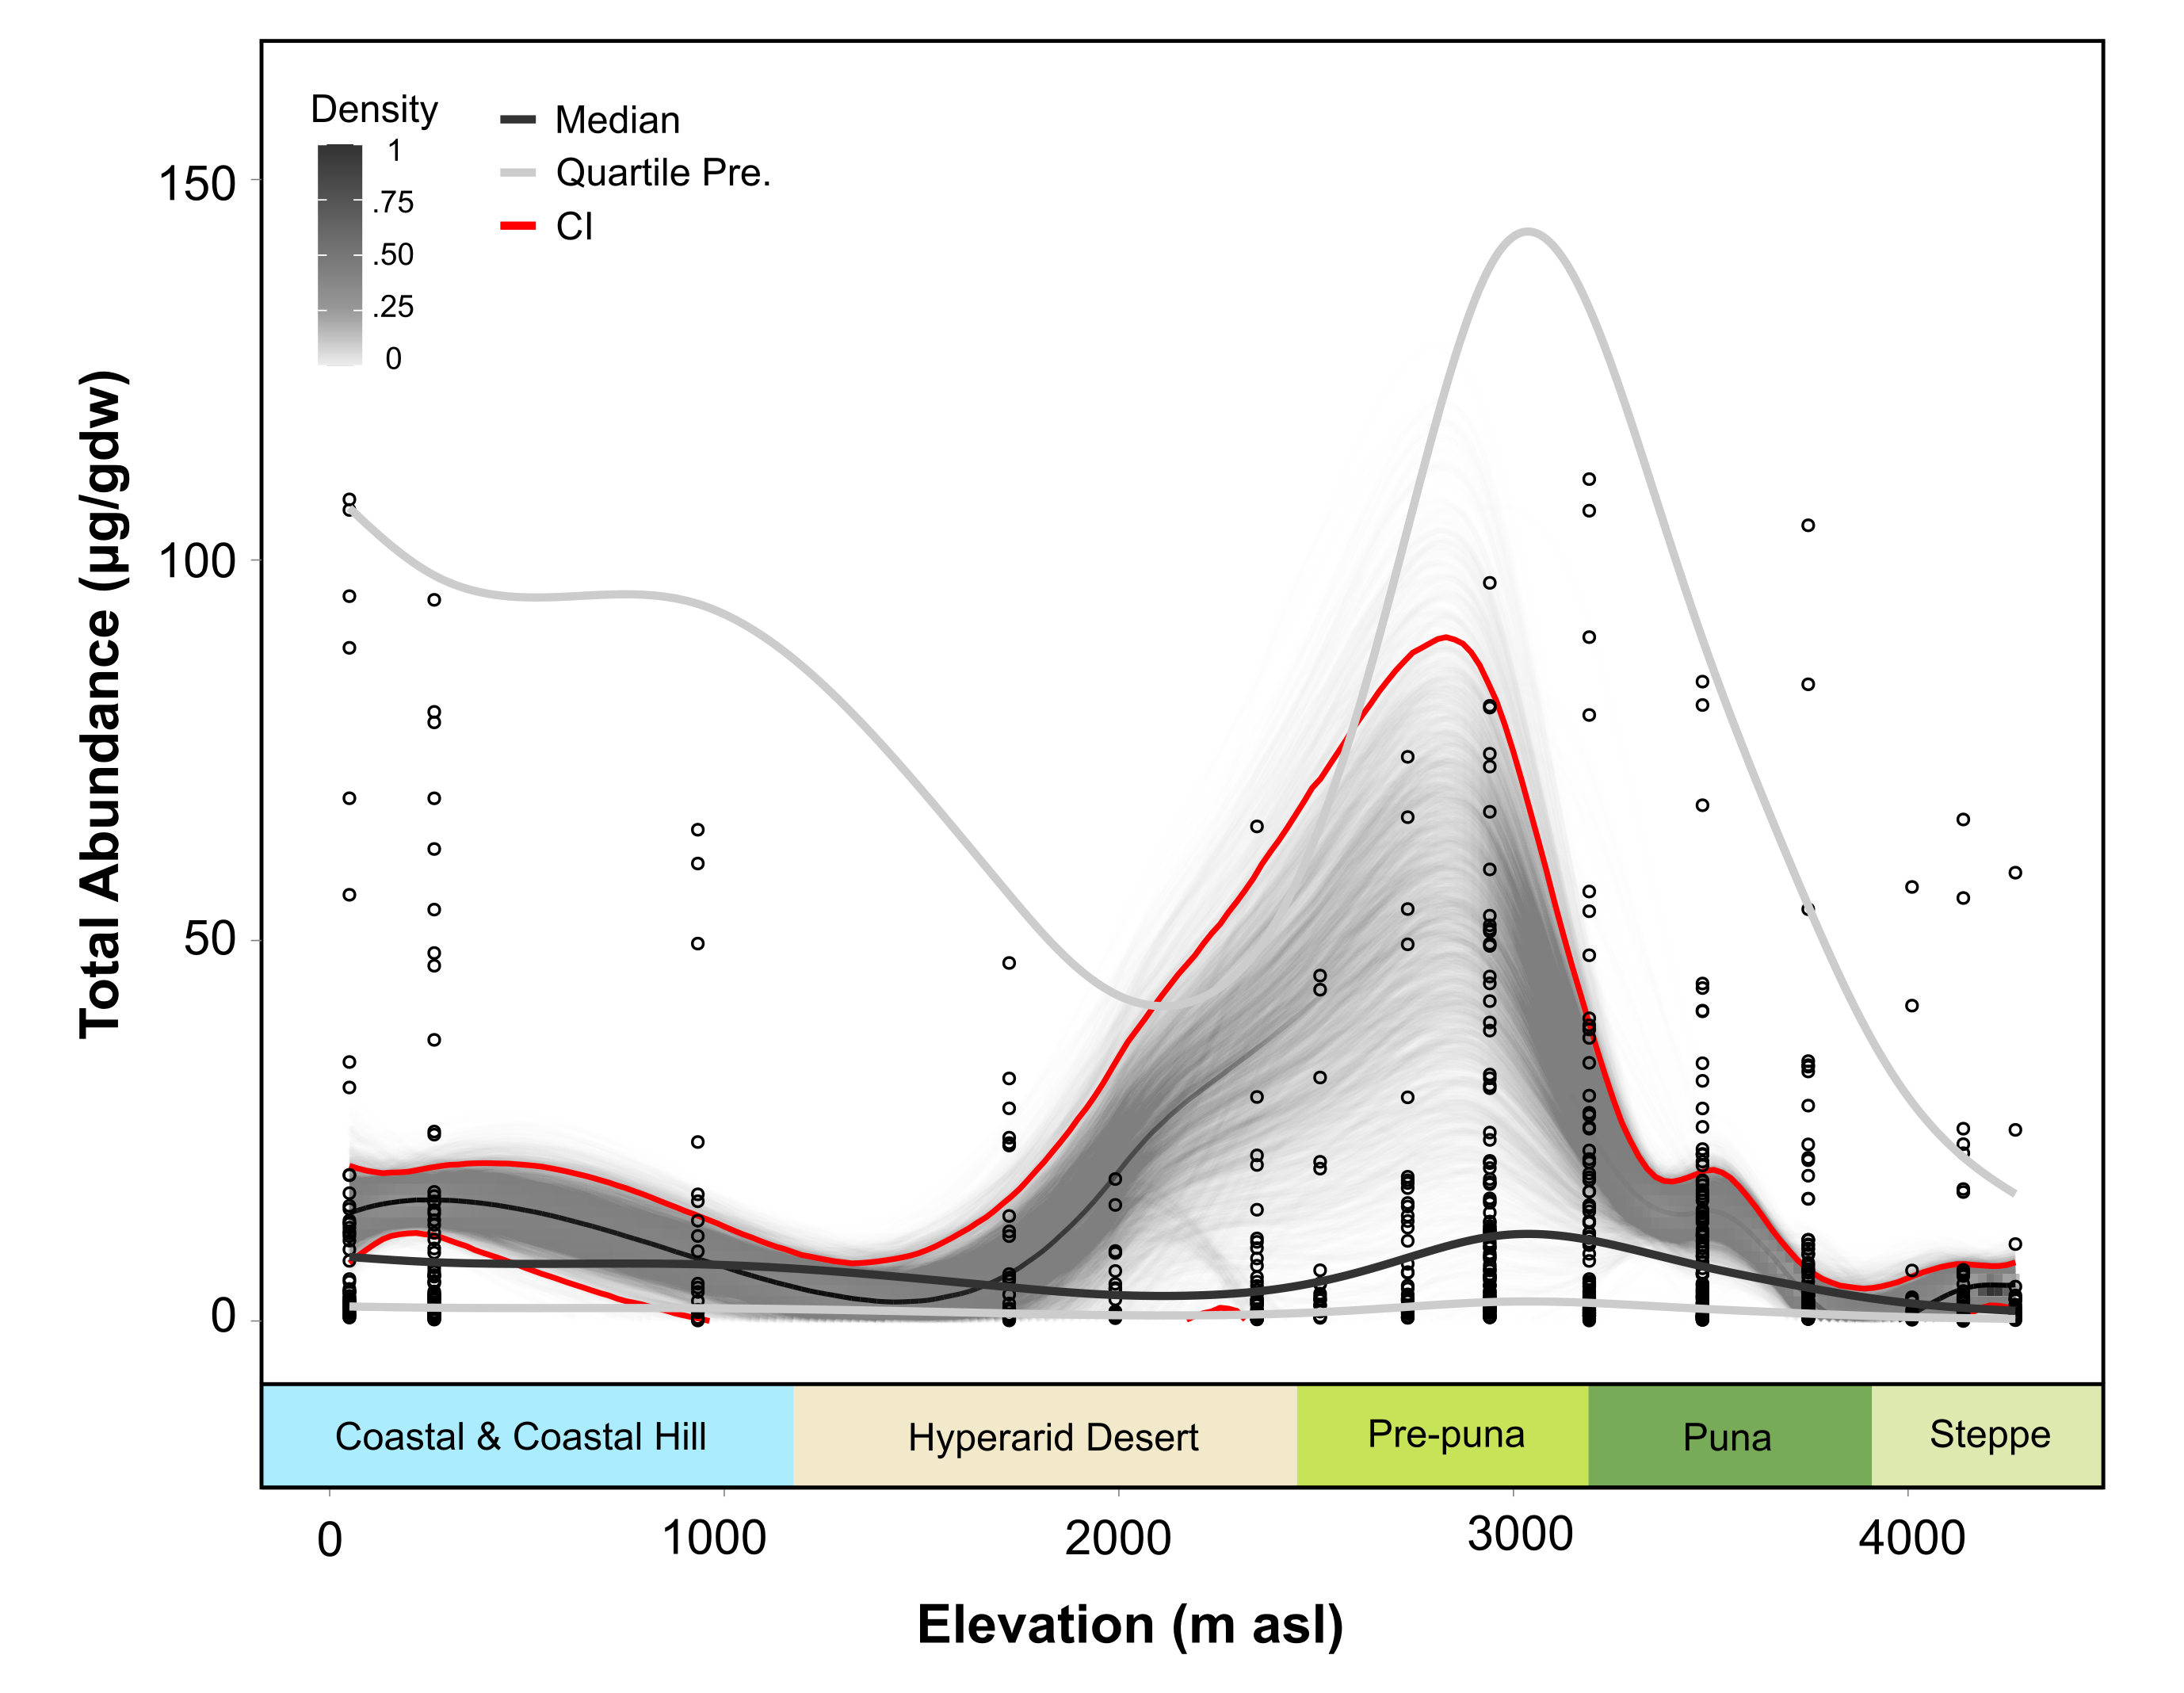
\includegraphics{images/Fig_2S.png}

}

\caption{Total abundances of individual long chains (\emph{n}-alkane and
\emph{n}-alkanoic acids) in leaf cuticular waxes along an environmental
gradient}

\end{figure}

\hypertarget{correlations-between-leaf-cuticular-waxes-and-the-temperature-and-precipitation-of-the-last-10-years-in-the-atacama-desert}{%
\subsection{Correlations between leaf cuticular waxes and the
temperature and precipitation of the last 10 years in the Atacama
Desert}\label{correlations-between-leaf-cuticular-waxes-and-the-temperature-and-precipitation-of-the-last-10-years-in-the-atacama-desert}}

To study the relationship between \emph{n}-alkyl lipid total abundances
and climate, we use the CR2MET gridded product which contains regional
precipitation, average temperature, minimum temperature and maximum
temperature values with a resolution of 0.05 degrees
(https://www.cr2.cl/datos-productos-grilados/). We calculated 19
bioclimatic layers that were used to evaluate different predictive
supervised models of \emph{n}-alkanes from no more than 3 input
parameters.

\begin{figure}

{\centering 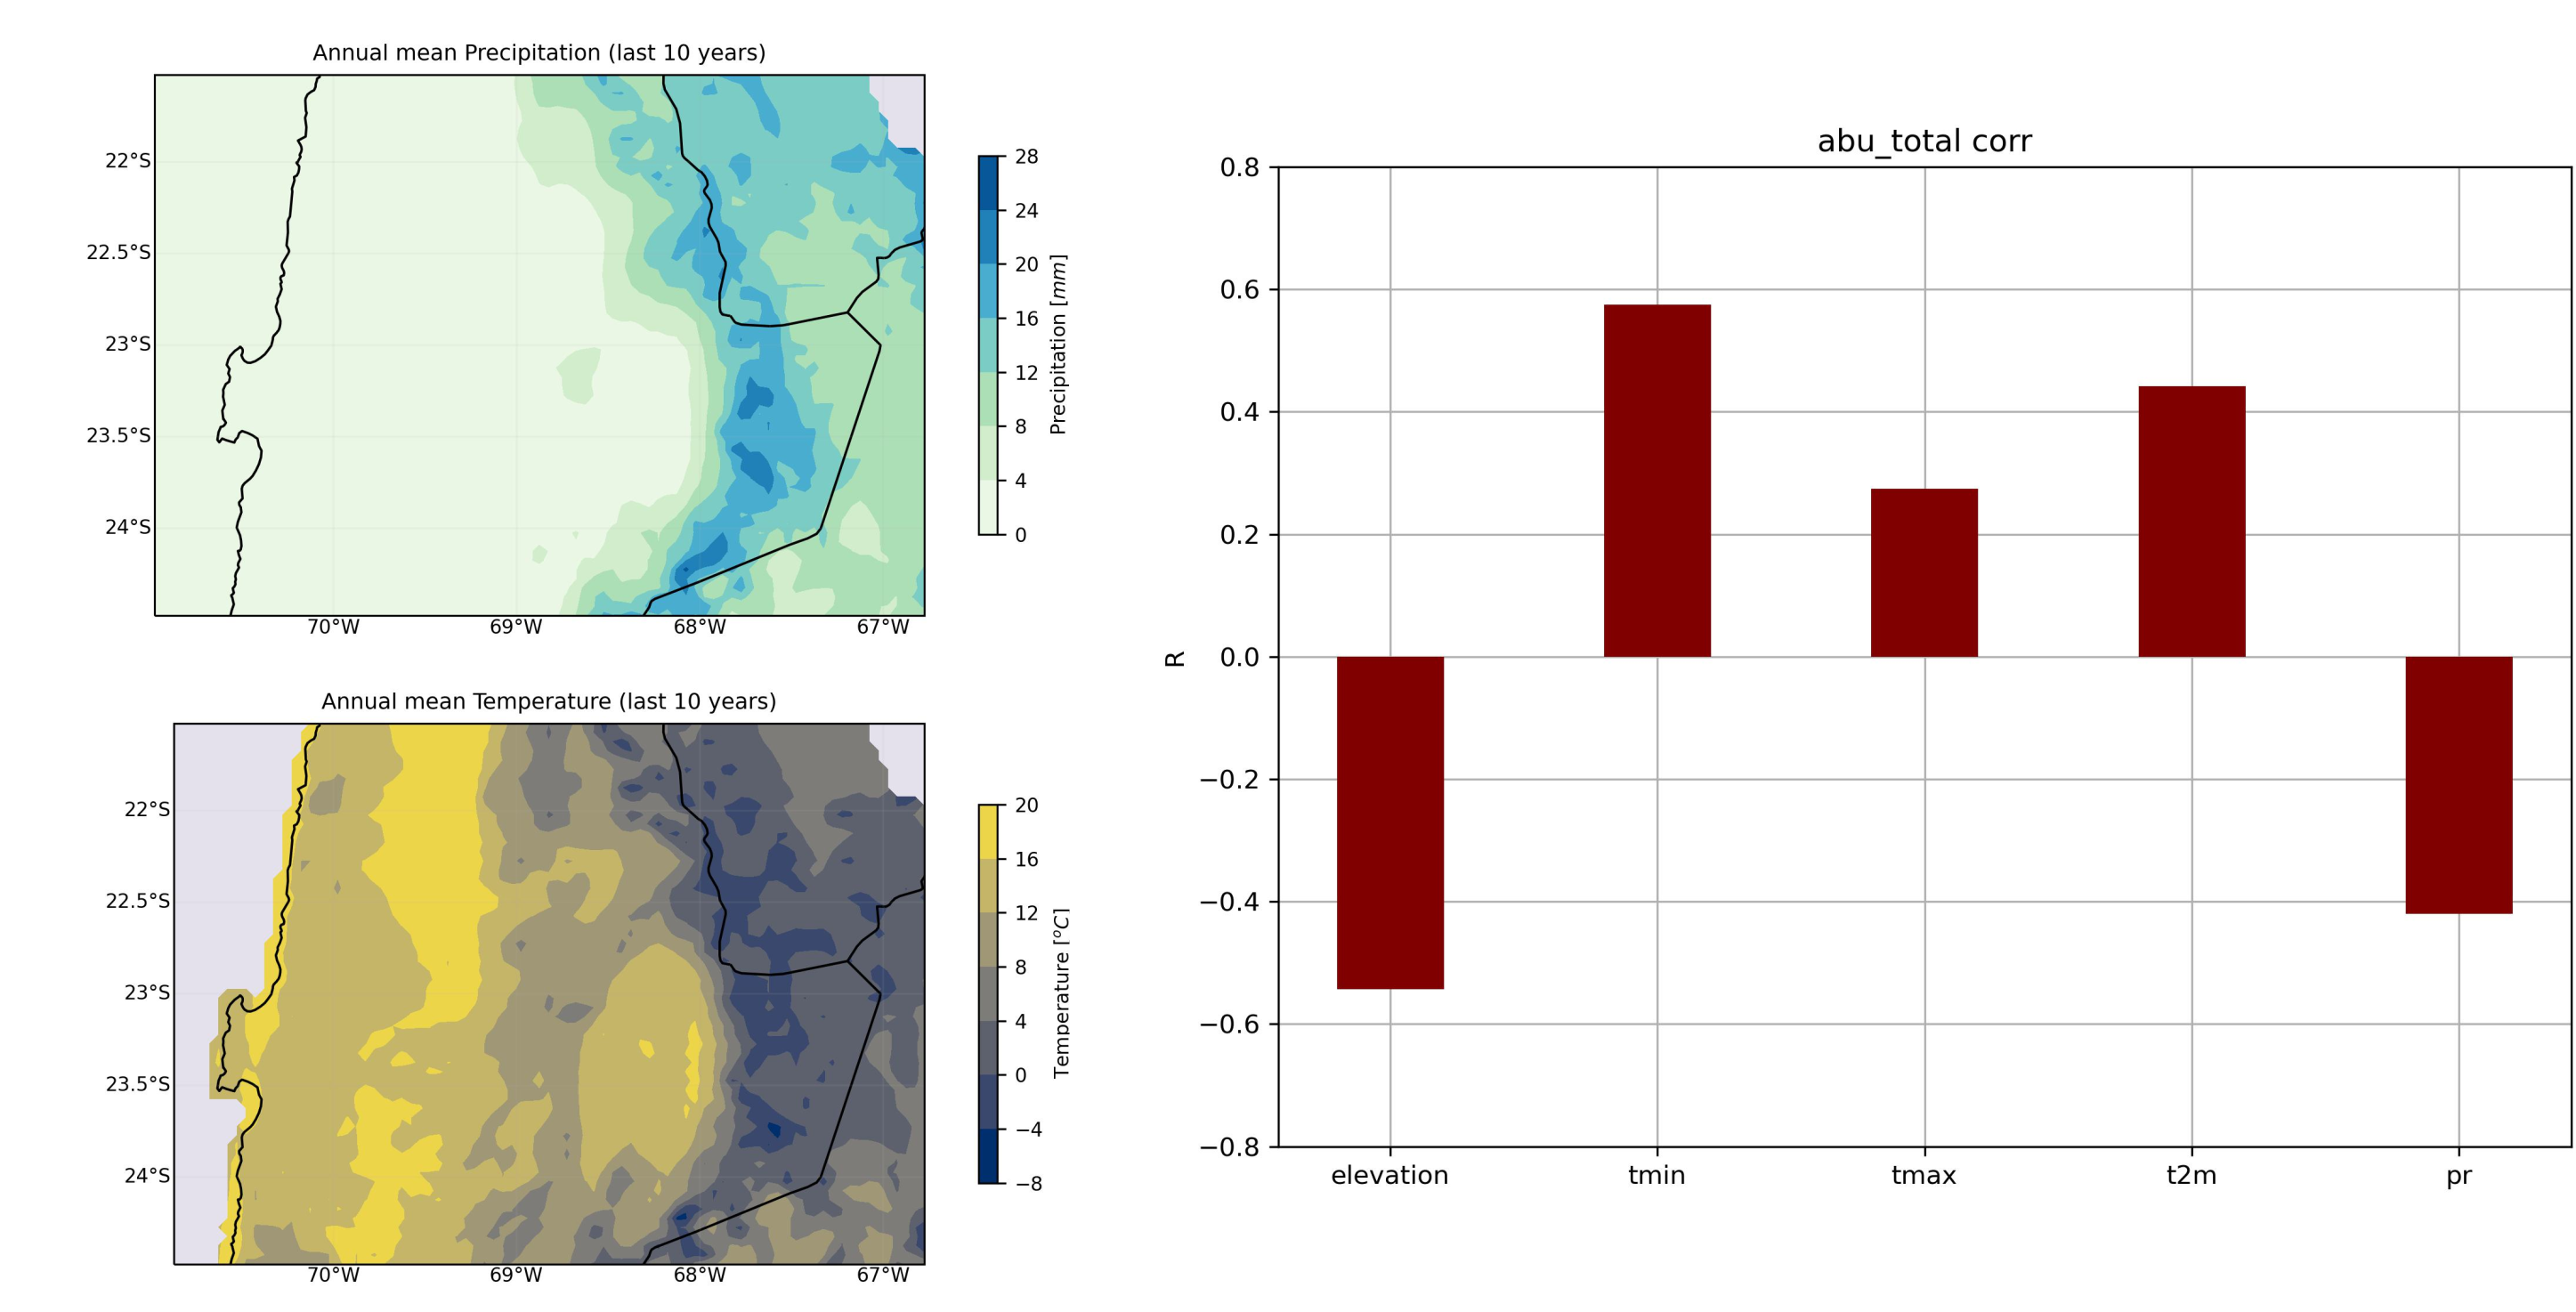
\includegraphics{images/Fig_3S.png}

}

\caption{Correlations between leaf waxes (\emph{n}-alkanes and
\emph{n}-alkanoic acids) and the temperature and precipitation of the
last 10 years in the Atacama Desert.}

\end{figure}

\begin{figure}

{\centering 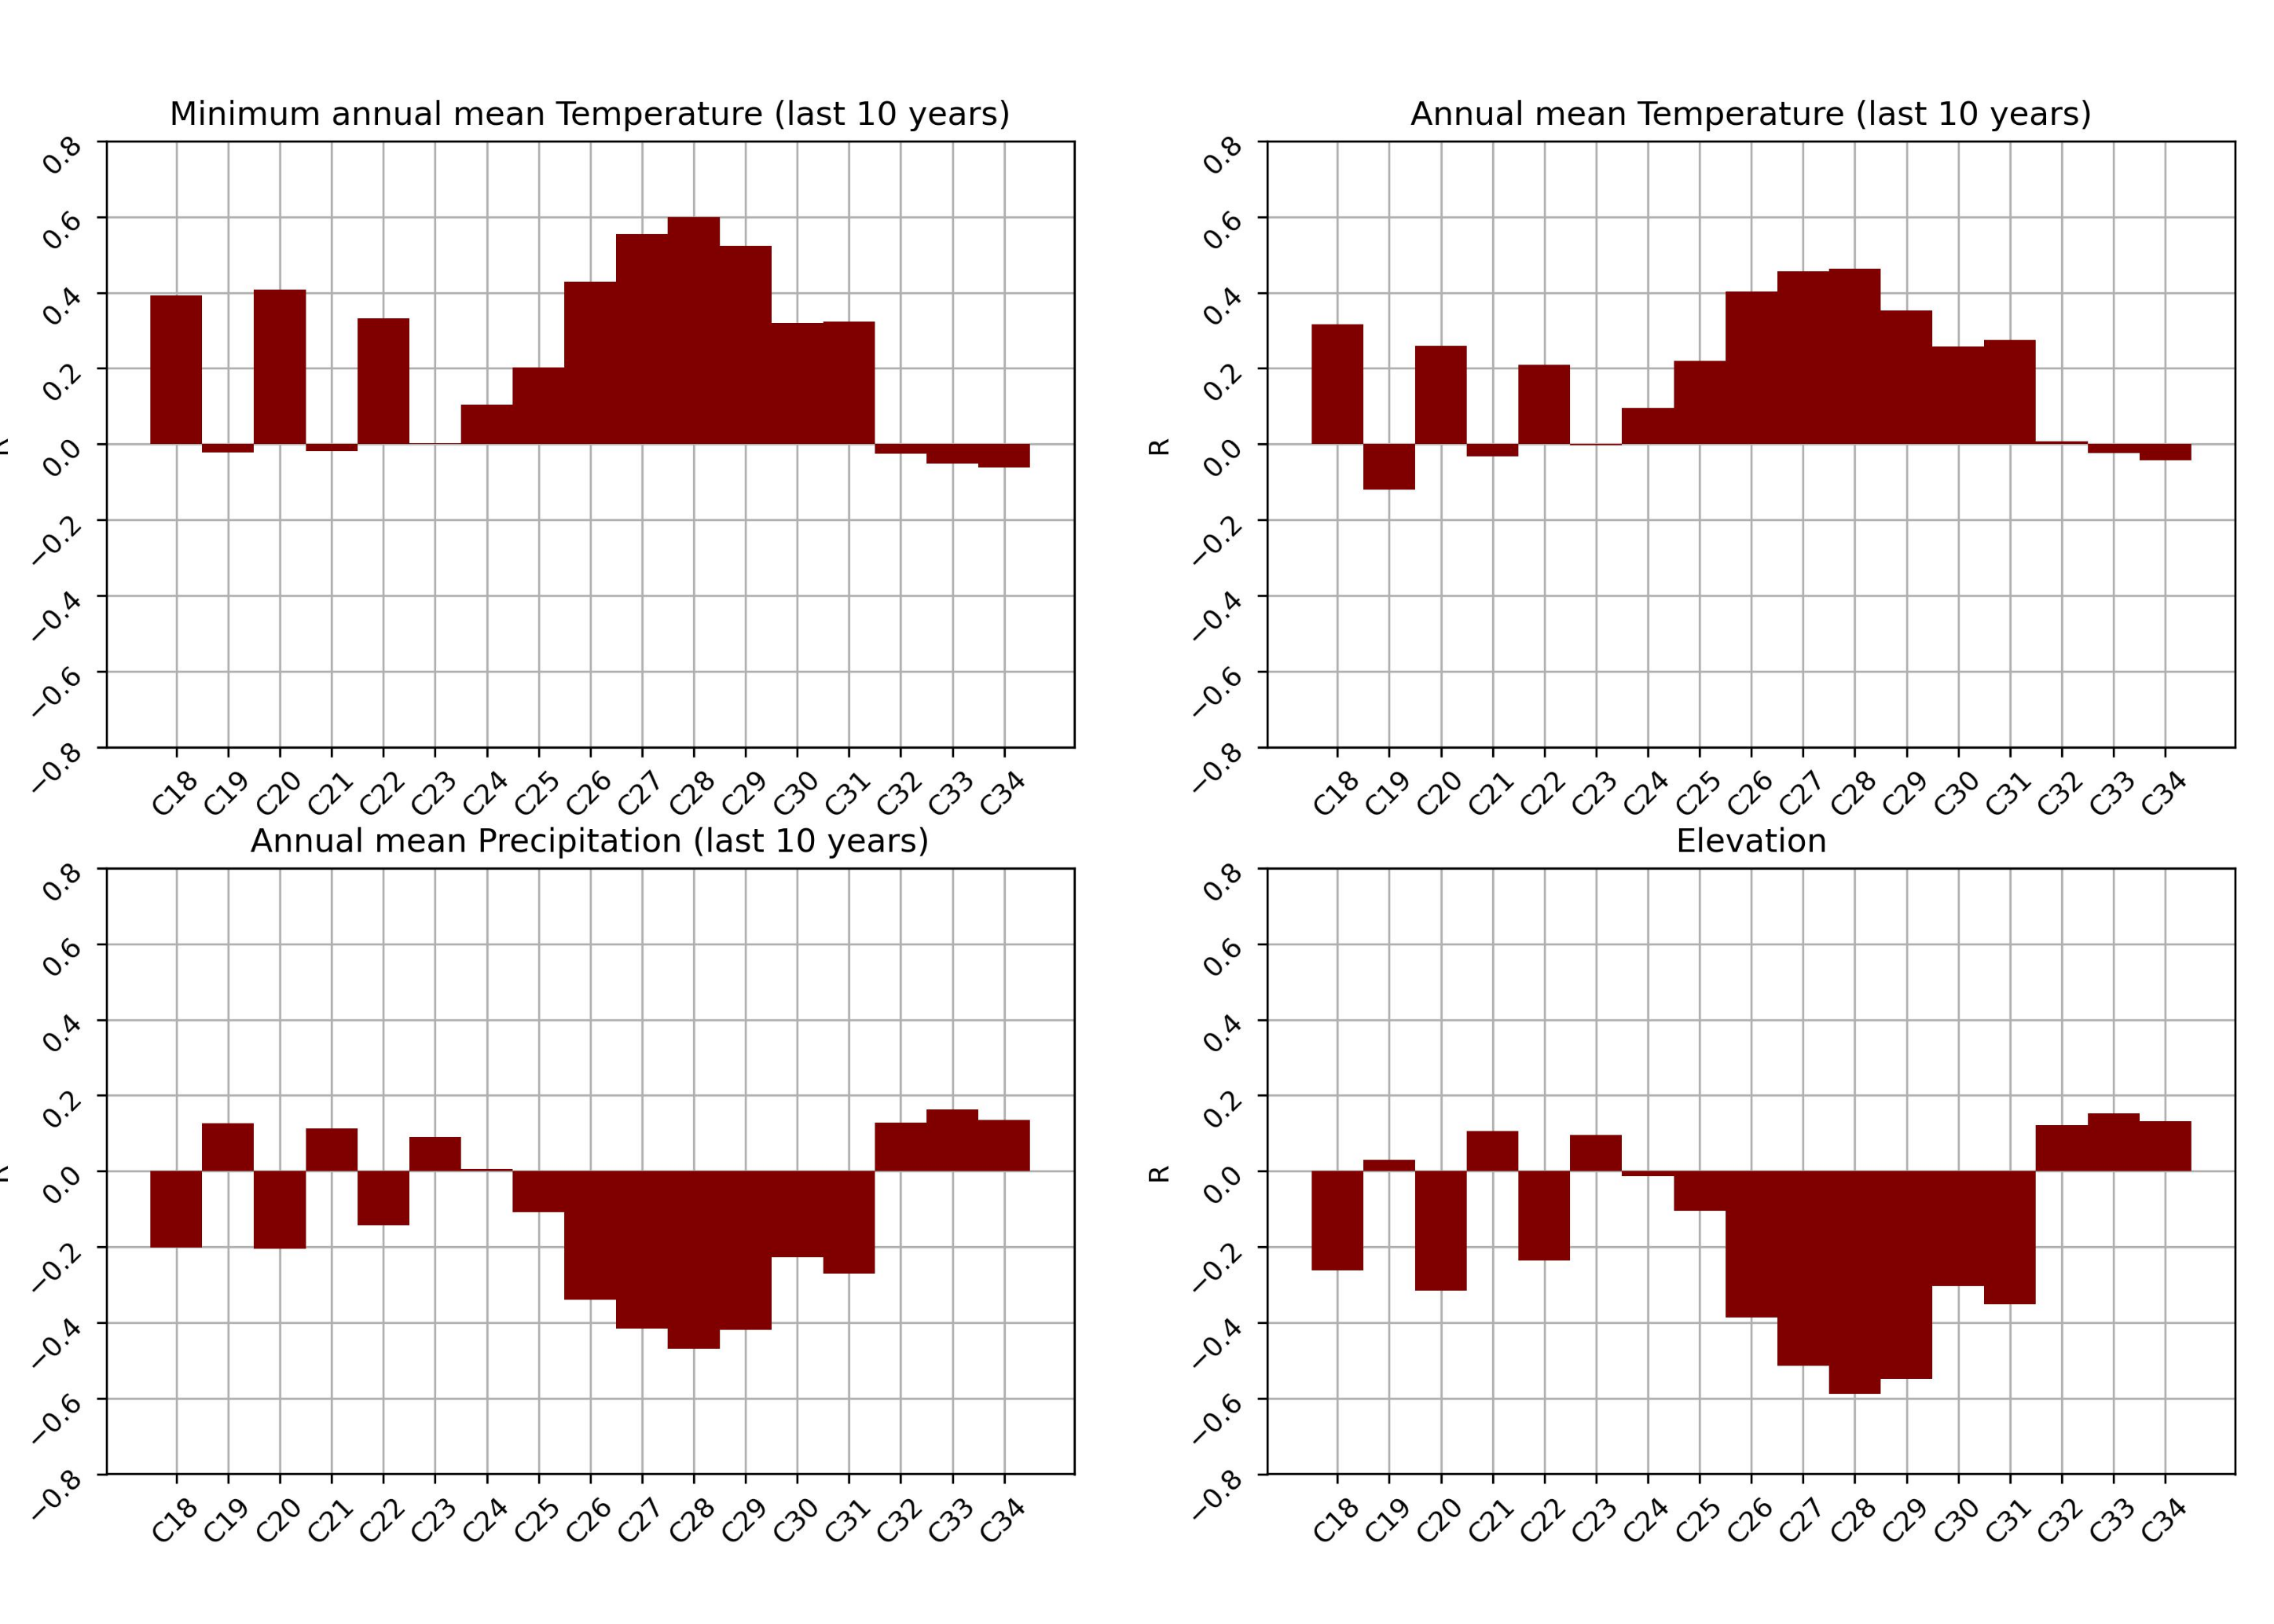
\includegraphics{images/Fig_4S.png}

}

\caption{Correlations between leaf waxes (\emph{n}-alkanes and
\emph{n}-alkanoic acids) and climate parameters from CR2MET gridded
product which contains regional precipitation, average temperature,
minimum temperature and maximum temperature values with a resolution of
0.05 degrees include of the last 10 years in the Atacama Desert}

\end{figure}

\begin{figure}

{\centering \includegraphics{images/Fig_5S.png}

}

\caption{Photographs of midden sites and collection. Note very low plant
abundance on alluvial landscapes and adjacent ignimbrite scarps. Middens
come from rock shelters along the scarp and from underneath boulders
strewn across the hillslope. \emph{n}-Alkanes in grasses and fecal
pellets of two paleomiddens from Quebrada Incahuasi (QIN237-B and
QIN214-B; 970 and 11780 a cal BP, respectively).}

\end{figure}

\begin{figure}

{\centering 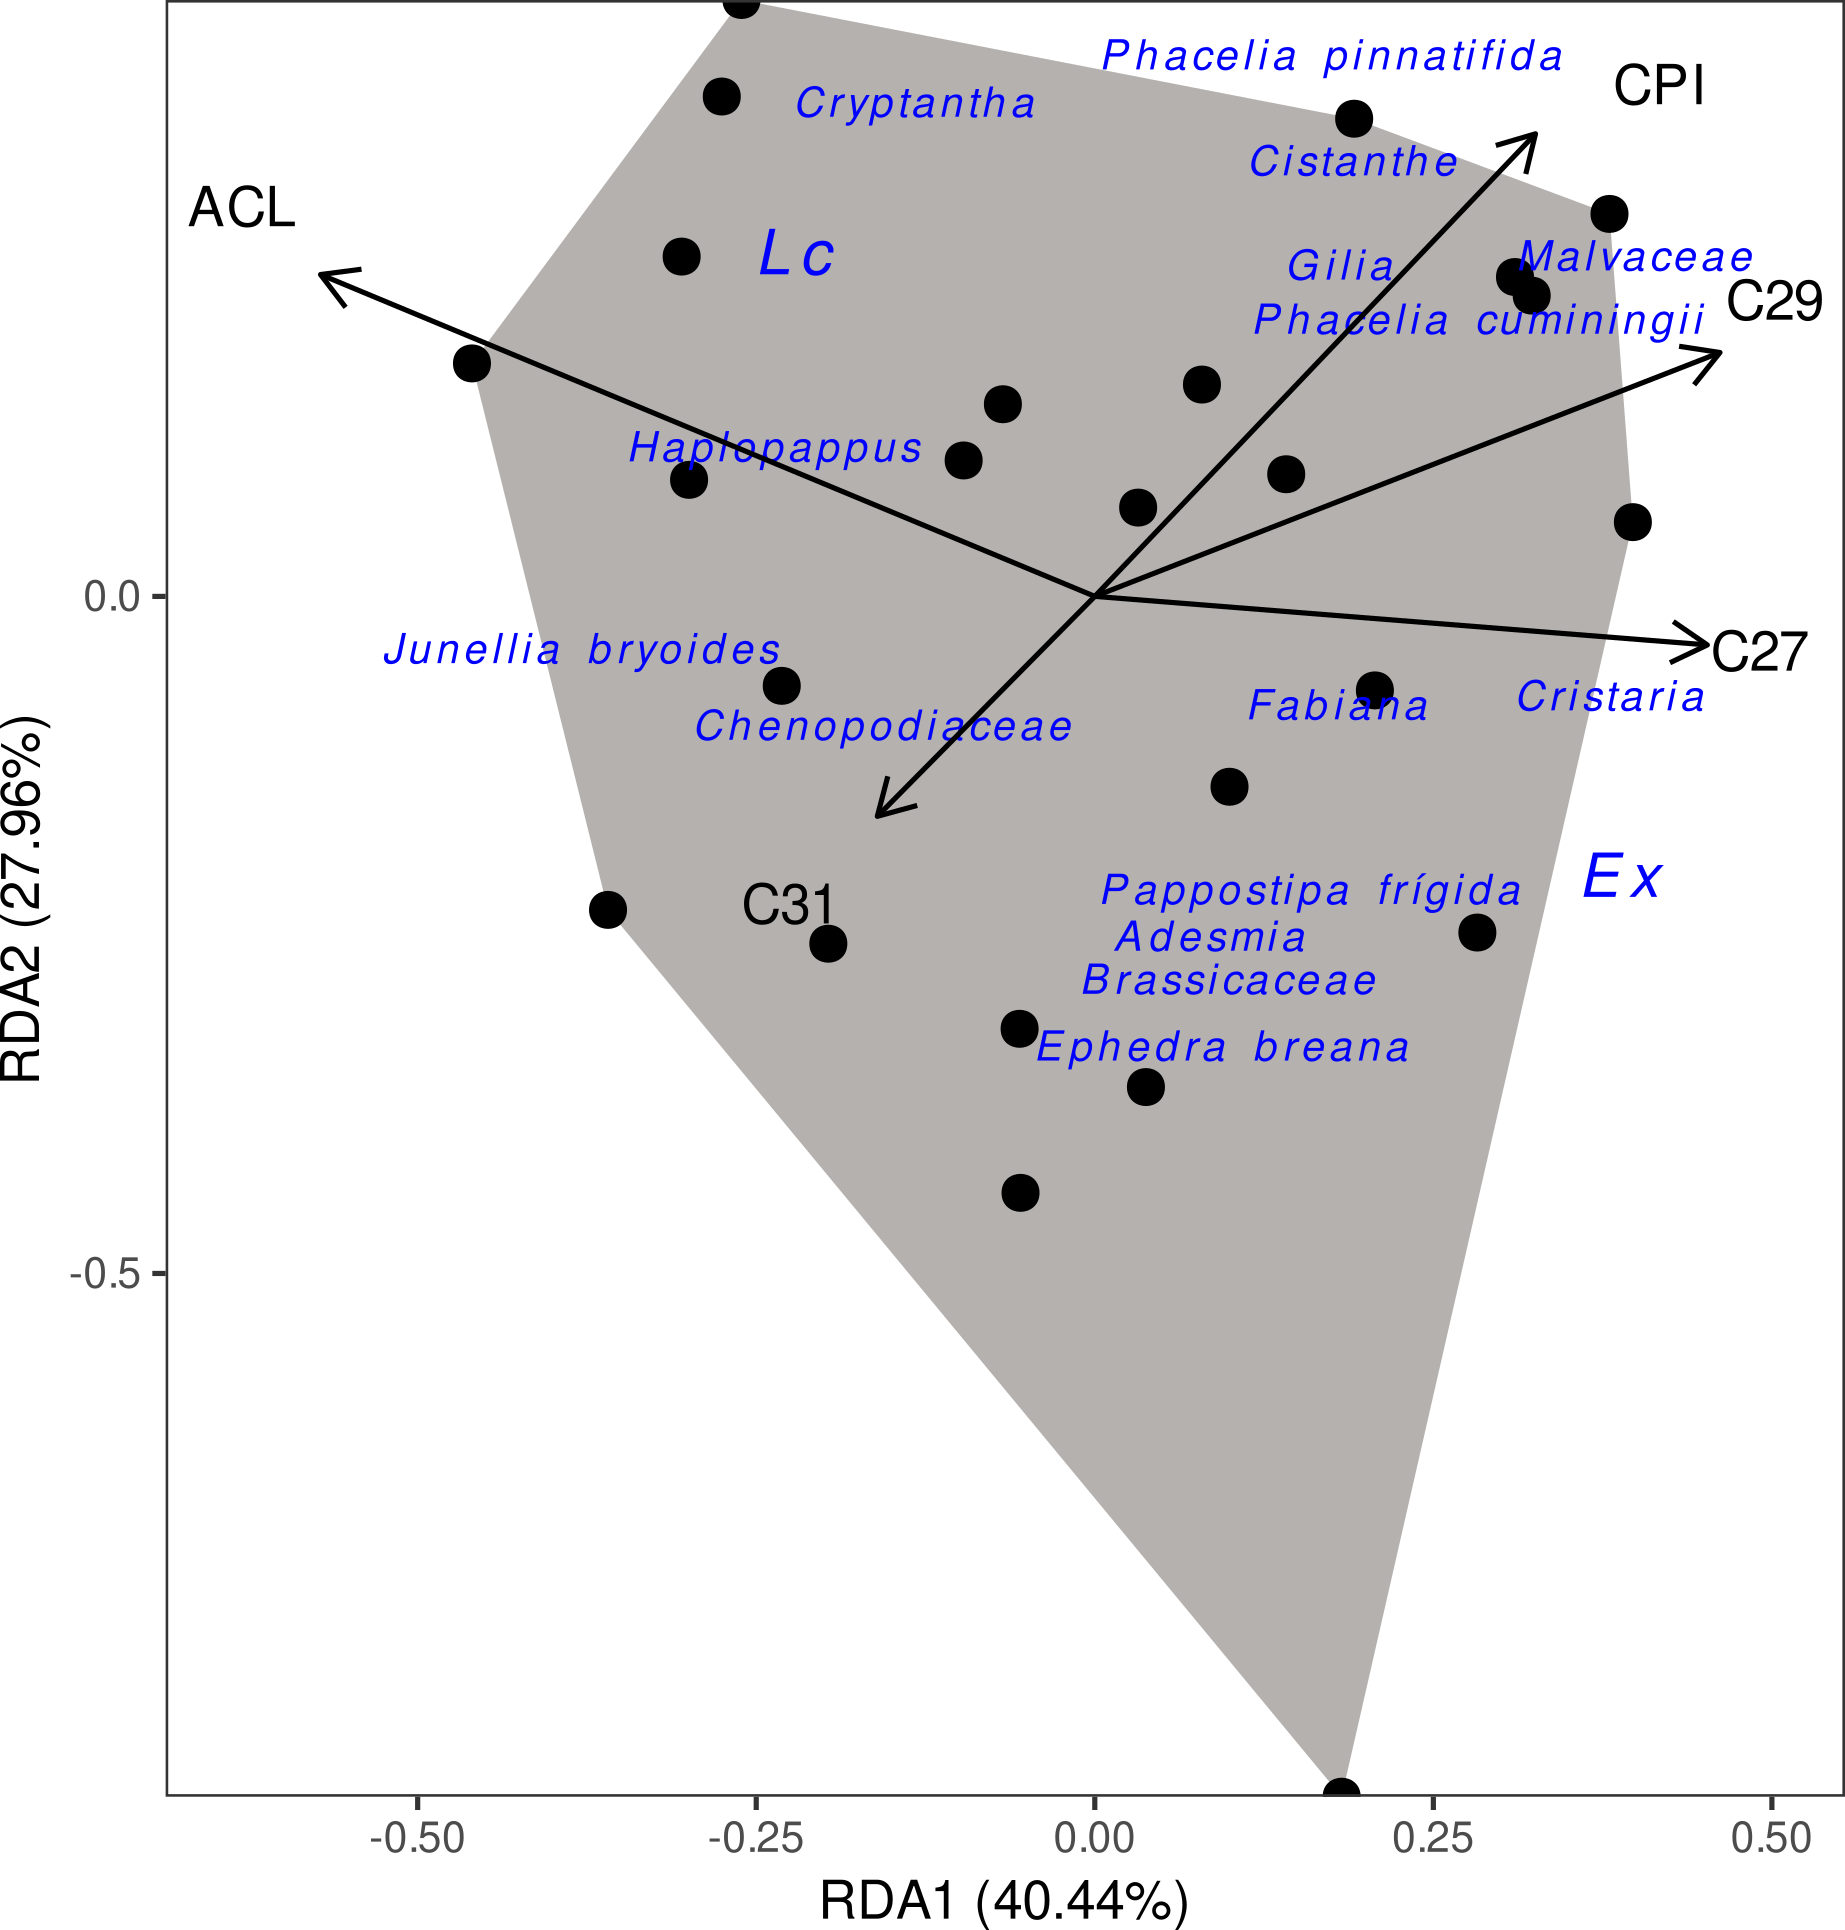
\includegraphics{images/Fig_6S.png}

}

\caption{Biplot for abundance of macrofossils and \emph{n}-alkanes (µg/g
dw) measured in fecal pellets from 25 paleomiddens spanning the last 17
cal kyr BP from Quebrada Incahuasi. Axis RDA1 explains 40,44\% of the
total variance, and axis RDA2 explains 28\% of the total variance. Both
RDA1 and RDA2 explain ca. 69\% of the total variance in the original
dataset and considering the outliers of the total content.
\emph{Phacelia cuminingii}, \emph{Phacelia pinnatifida}, \emph{Junellia
bryoides}, \emph{Cistanthe} sp., \emph{Ephedra americana}, \emph{Gilia}
sp., \emph{Haplopappus} sp., \emph{Cryptantha} sp., \emph{Baccharis aff.
tola}, \emph{Brassicaceae aff. Atacama nivea}, \emph{Pappostipa
frigida}, \emph{Cristaria} sp., \emph{Fabiana} sp.,
\emph{Chenopodiaceae}, \emph{Malvaceae}, \emph{Adesmia} sp., local
(\emph{Lc}) and extra-local (\emph{Ex}) specie were used to generate the
RDA.}

\end{figure}

\hypertarget{tables}{%
\section{Tables}\label{tables}}

\hypertarget{tbl-1}{}
\setlength{\LTpost}{0mm}
\begin{longtable}{crrrrrrr}
\caption{\label{tbl-1}Summary statistics of leaf wax n-alkanes and n-alkanoic acids abundance }\tabularnewline

\toprule
wax & n & mean\_abundance & sd\_abundance & median\_CPI & mad\_CPI & median\_ACL & mad\_ACL \\ 
\midrule
\multicolumn{8}{l}{Middens} \\ 
\midrule
n-Alkanes & 28 & 335.41158 & 239.295619 & 18.461910 & 5.44384077 & 29.12240 & 0.40321519 \\ 
\midrule
\multicolumn{8}{l}{Surface Sediment} \\ 
\midrule
FAMEs & 3 & 117.31495 & 52.518303 & 11.031963 & 2.61510956 & 24.24743 & 0.06611670 \\ 
n-Alkanes & 6 & 10.44854 & 5.074585 & 9.137297 & 1.97561310 & 25.92026 & 0.63028168 \\ 
\midrule
\multicolumn{8}{l}{Aloysia deserticola} \\ 
\midrule
FAMEs & 3 & 215.48935 & 54.049054 & 2.103820 & 0.39076411 & 28.55057 & 1.03106886 \\ 
n-Alkanes & 3 & 210.95087 & 24.434815 & 5.846915 & 0.38010692 & 29.48836 & 0.06113192 \\ 
\midrule
\multicolumn{8}{l}{Atriplex imbricata} \\ 
\midrule
FAMEs & 8 & 286.81215 & 218.972281 & 9.905374 & 3.76662109 & 26.03645 & 1.45313837 \\ 
n-Alkanes & 8 & 141.81598 & 75.485040 & 18.360459 & 5.45399686 & 27.49319 & 1.33151406 \\ 
\midrule
\multicolumn{8}{l}{Cristaria integerrima} \\ 
\midrule
FAMEs & 1 & 91.15866 & NA & 5.796533 & 0.00000000 & 25.69106 & 0.00000000 \\ 
n-Alkanes & 1 & 339.86887 & NA & 12.427098 & 0.00000000 & 27.07403 & 0.00000000 \\ 
\midrule
\multicolumn{8}{l}{Ephedra sp.} \\ 
\midrule
FAMEs & 2 & 913.46960 & 992.635678 & 12.947829 & 5.88178808 & 27.41692 & 0.65451011 \\ 
n-Alkanes & 2 & 70.36172 & 61.312032 & 8.223281 & 4.45716247 & 28.16296 & 1.57494303 \\ 
\midrule
\multicolumn{8}{l}{Haplopappus rigidus} \\ 
\midrule
FAMEs & 2 & 236.03747 & 278.924811 & 7.319356 & 4.82673389 & 26.59827 & 2.17361163 \\ 
n-Alkanes & 4 & 207.11847 & 58.632182 & 11.599664 & 2.34967561 & 26.27221 & 1.19129699 \\ 
\midrule
\multicolumn{8}{l}{Jarava frigida} \\ 
\midrule
FAMEs & 5 & 115.10662 & 46.286095 & 13.141929 & 3.20422685 & 28.58114 & 0.83168444 \\ 
n-Alkanes & 7 & 97.38671 & 116.663841 & 13.301322 & 10.84899836 & 28.85701 & 0.78851809 \\ 
\midrule
\multicolumn{8}{l}{Junellia seriploide} \\ 
\midrule
FAMEs & 2 & 375.88277 & 333.235859 & 8.293965 & 1.64251416 & 24.91031 & 0.12623827 \\ 
n-Alkanes & 2 & 79.04812 & 21.342944 & 11.519030 & 2.02671942 & 28.60531 & 0.05760277 \\ 
\midrule
\multicolumn{8}{l}{Nolana aplocaryoides} \\ 
\midrule
FAMEs & 1 & 142.39482 & NA & 6.381062 & 0.00000000 & 25.15165 & 0.00000000 \\ 
n-Alkanes & 1 & 332.41291 & NA & 23.721943 & 0.00000000 & 28.85614 & 0.00000000 \\ 
\midrule
\multicolumn{8}{l}{Perityle emoryi} \\ 
\midrule
n-Alkanes & 1 & 789.95012 & NA & 14.463342 & 0.00000000 & 28.92927 & 0.00000000 \\ 
\midrule
\multicolumn{8}{l}{Sp2} \\ 
\midrule
FAMEs & 1 & 227.98959 & NA & 14.979941 & 0.00000000 & 24.10160 & 0.00000000 \\ 
n-Alkanes & 1 & 407.16792 & NA & 56.383496 & 0.00000000 & 29.00538 & 0.00000000 \\ 
\midrule
\multicolumn{8}{l}{Sp3} \\ 
\midrule
FAMEs & 1 & 231.15961 & NA & 8.105427 & 0.00000000 & 28.57253 & 0.00000000 \\ 
n-Alkanes & 1 & 184.31794 & NA & 9.483458 & 0.00000000 & 28.20043 & 0.00000000 \\ 
\midrule
\multicolumn{8}{l}{Tiquilia atacamensis} \\ 
\midrule
FAMEs & 3 & 107.77041 & 53.135379 & 9.943925 & 0.03941876 & 22.93231 & 0.47453506 \\ 
n-Alkanes & 3 & 89.80569 & 30.591602 & 8.440672 & 0.61098165 & 28.96094 & 0.16799931 \\ 
\bottomrule
\end{longtable}
\begin{minipage}{\linewidth}
TA [ug/gdw]; Total Abundance\\
TA mad; median absolute deviation form Total Abundance\\
\end{minipage}

\hypertarget{supplementary-discussion}{%
\section{Supplementary Discussion}\label{supplementary-discussion}}

Compared to other deserts, most of the plants in the south-central
Atacama landscapes incorporate atmospheric \(CO_{2}\) through the
\(C_{3}\) photosynthetic pathway ---although there are several CAM
species \citep{ehleringerCarbonIsotopeRatios1998}. Only a few perennial
shrubs and summer annual herbs \(C_{4}\) grow in higher temperature and
moisture zones. In the Steppe, species composition was mainly of the
Poaceae family, dominated by \emph{Pappostipa frigida} which shows high
leaf waxes abundance of chain length
\emph{n}-\(C_{28}\)/\emph{n}-\(C_{29}\) and
\emph{n}-\(C_{30}\)/\emph{n}-\(C_{31}\) (Figure 1S).
\citet{diefendorfExtractingMostTerrestrial2017} describe in \(C_{3}\)
graminoids that the dominant \emph{n}-alkane was \emph{n}-\(C_{31}\),
followed by \emph{n}-\(C_{33}\) and \emph{n}-\(C_{29}\). In the Puna, in
addition to \emph{P. frigida}, the landscape was dominated by the
species \emph{H. rigidus} and \emph{J. seriphioides}. These species
containing high abundances of \emph{n}-\(C_{25}\)/\emph{n}-\(C_{28}\)
and \emph{n}-\(C_{21}\)/\emph{n}-\(C_{22}\), respectively (Figure 1S).
In the Prepuna, the species \emph{Atriplex imbricata} (Amaranthaceae),
\emph{Aloysia deserticola} and \emph{Haplopappus rigidus} are
predominant. The \(C_{4}\) sub-shrub \emph{A. imbricata} showed a wide
distribution along the altitudinal gradient (between 1,700 and 3,200 m
asl) and higher abundances of \emph{n}-\(C_{28}\)/\emph{n}-\(C_{27}\)
chain length followed by \emph{n}-\(C_{24}\)/\emph{n}-\(C_{25}\),
\emph{n}-\(C_{28}\)/\emph{n}-\(C_{29}\) and
\emph{n}-\(C_{30}\)/\emph{n}-\(C_{31}\) (Figure 1S). In addition, the
abundance of \emph{n}-alkanes in \emph{A. imbricata} presents
significantly correlates with elevation (p \textless{} 0.001; \(R^{2}\)=
0.8, Figure 2S). In Africa, Australia, and North America, \(C_{4}\)
plants show much higher abundances of the alkanes \emph{n}-\(C_{29}\),
\emph{n}-\(C_{31}\) and \emph{n}-\(C_{33}\)
\citep{carrLeafWaxNalkane2014, feakinsProductionLeafWax2016, garcinReconstructingC3C42014, howardModellingLeafWax2018, vogtsDistributionPatternsStable2009}.
\emph{A. deserticola} contains a higher abundance of \emph{n}-alkane
\emph{n}-\(C_{31}\) followed by \emph{n}-\(C_{29}\), and in general,
shows lower abundances of \emph{n}-alkanoic acids compared to
\emph{n}-alkanes. \emph{H. rigidus} shows a higher abundance of
\emph{n}-\(C_{25}\). In the hyperarid desert, we found only two species,
\emph{T. atacamensis} and \emph{A. imbricata}. \emph{T. atacamensis}
showed a clear dominance of \emph{n}-\(C_{22}\)/\emph{n}-\(C_{29}\).
This asymmetric distribution between \emph{n}-alkanes and
\emph{n}-alkanoic acids chain length abundances could be a structural
adaptation to extreme aridity ---generating higher abundances of short-
and medium- \emph{n}-alkanoic acids chain length as precursors to other
aliphatic compounds of cuticular waxes--- thereby favoring hydrophobic
conditions that reduce water loss
\citep{bushLeafWaxNalkane2013, contrerasLeafWaxComposition2022, mackovaPlantResponseDrought2013, shepherdEffectsStressPlant2006}.
On the coast, \emph{C. integerrima} and \emph{N. aplocaryoides} were the
dominant species with chain lengths of \emph{n}-\(C_{27}\) and
\emph{n}-\(C_{29}\), respectively. However, in the field, we found low
species abundance and richness. These data generally support the idea
that the dominant \emph{n}-alkane chain abundances have strong
species-specific chemotaxonomic signatures
\citep{cerda-penaMolecularNalkylLeaf2020}.


\renewcommand\refname{References}
  \bibliography{bibliography.bib}


\end{document}
